% This work is licensed under the Creative Commons Attribution-NonCommercial 4.0 International License.
% To view a copy of this license, visit http://creativecommons.org/licenses/by-nc/4.0/
% or send a letter to Creative Commons, PO Box 1866, Mountain View, CA 94042, USA.

% !TEX TS-program = xelatex

\documentclass[../Main/chem371-notes.tex]{subfiles}

\setcounter{chapter}{4}
\begin{document}

\chapter{Basis Sets}

In the previous chapter we introduced the Hartree--Fock method. 
The goal of this chapter is to discuss some practical aspects of how Hartree--Fock computations actually run on a computer and the way the are approximated.
We will encounter the idea of using a linear combination of basis functions to approximate the orbitals $\varphi(\mathbf{r})$ in systematically improvable way.
Lastly, we will look at some applications of these ideas.

\section{Exact solutions to the Schr\"{o}dinger equation for the hydrogen atom}
As it was mentioned earlier, we know exact solutions of the Schr\"{o}dinger only for a handful of models.
An example that should be familiar to you is the hydrogen atom.
For this system, the solutions are known to depend on three quantum numbers $n$, $l$, and $m_l$, and that the energy levels (eigenvalues) are given by (in atomic units)
\begin{iequation}
E_n = - \frac{1}{2 n^2}  \, E_\mathrm{h}, \quad n = 1, 2, \ldots
\end{iequation}
The wave function $\psi_{nlm_l}$ is usually expressed in \emph{spherical coordinates} ($r, \theta, \phi$)\mnote{
If you are curious, spherical coordinates are connected to Cartesian coordinates via the following equations
\begin{align*}
x & =  r \sin \theta \cos \phi, \\
y & =  r \sin \theta \sin \phi, \\
z & =  r \cos \theta
\end{align*}
\centering{
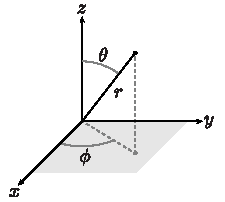
\includegraphics[width=2.0in]{img/spherical_coordinates.pdf}}
\captionof{figure}{Definition of the spherical coordinates $r$, $\theta$, and $\phi$.}
\label{fig:rigidrotor:spherical}
}
 as a product of a function that depends on the electron distance $R_{nl}(r)$ and a term that depends on the angles $\theta$ and $\phi$, which we write as $Y_l^{m_l}(\theta,\phi)$
\begin{equation}
\psi_{nlm_l}(r,\theta,\phi) = R_{nl}(r) Y_l^{m_l}(\theta,\phi)
\end{equation}
For example, the wave function for the  ground state of hydrogen, the 1s orbital, is given by
\begin{equation}
\mathrm{1s} = \psi_{1,0,0}(r,\theta,\phi) = R_{1,0}(r) Y_0^0(\theta,\phi) = 2 e^{-r} \frac{1}{\sqrt{4\pi}} = \frac{1}{\sqrt{\pi}} e^{-r}
\end{equation}
while the 2p$_{z}$ orbital is given by
\begin{align}
\mathrm{2p}_{z} &= \psi_{2,1,0}(r,\theta,\phi) = R_{2,1}(r) Y_1^{0}(\theta,\phi) =
\frac{1}{4\sqrt{2 \pi}}   r e^{-r/2} \cos \theta.
\end{align}

When we turn to more complicated systems, like atoms with more than one electron and molecules, the Schr\"{o}dinger equation becomes intractable and we have to turn to approximate numerical methods to solve it (recall Dirac's quote on this point).
This is what we will look into in the next section.

\section{Bases, basis vectors, and basis functions}

\mfigure{
\centering{
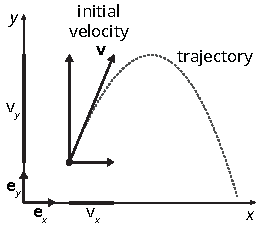
\includegraphics[width=1.75in]{img/trajectory.pdf}}
\captionof{figure}{The trajectory of a particle with initial velocity vector $\mathbf{v} = (v_x, v_y)$.
This vector may be decomposed in the basis of orthogonal unit vectors $\mathbf{e}_x$ and $\mathbf{e}_y$ as $\mathbf{v} = v_x \mathbf{e}_x + v_y \mathbf{e}_y$.}
\label{fig:2dtraj}
}

An important concept when constructing numerical approximations is that of a basis.
To build some intuition about the concept of a basis you can think back to your introductory physics courses and Newton's equations.
Consider the problem of describing the trajectory of a particle under the effect of gravity.
To solve this problem you need to specify the position and initial velocity of the particle.
The position can be specified by the $x$ and $y$ coordinates, and the initial velocity by the velocity in $x$ and $y$ directions ($v_x, v_y$).
These quantities are essentially vectors, which we indicate with the symbols $\mathbf{r} = (x,y)$ and $\mathbf{v} = (v_x,v_y)$.
Figure~\ref{fig:2dtraj} shows the position and velocity vectors.

Every vector can be written as a \emph{linear combination}\mnote{
A linear combination of vectors/functions/etc. ($f_i$) is a sum
\begin{equation*}
f_1 c_1 + f_2 c_2 + \ldots + f_K c_K
\end{equation*}
where the quantities $c_1, c_2, \ldots$ are numbers (they can be real or complex).
} of vectors that are linearly independent and span the full space, which we call a \emph{basis}.
For example, the velocity vector $\mathbf{v}$ can be expressed as a sum of a component pointing in the $x$ direction ($\mathbf{e}_x$) and one pointing in the $y$ direction ($\mathbf{e}_y$)
\begin{equation}
\mathbf{v} = v_x \mathbf{e}_x + v_y \mathbf{e}_y, \text{ with } \mathbf{e}_x = (1,0) \text{ and } \mathbf{e}_y = (0,1)
\end{equation}
The vectors $\mathbf{e}_x$ and $\mathbf{e}_y$ are called a basis, because any vector in two dimensions $\mathbf{a}$ can be written as a sum of coefficients multiplied by the basis vectors
\begin{equation}
\mathbf{a} = a_x \mathbf{e}_x + a_y \mathbf{e}_y
\end{equation}
The vectors $\mathbf{e}_x$ and $\mathbf{e}_y$ have another special property: they are orthogonal, which means that their dot product is zero\mnote{A basis can have orthogonal  or nonorthogonal vectors. However, bases that are orthogonal are typically preferred.}
\begin{equation}
 \mathbf{e}_x \cdot \mathbf{e}_y = 0.
\end{equation}

In the more general case, the velocity is a three dimensional vector, and must be described as a sum of three terms
\begin{equation}
\mathbf{v} = v_x \mathbf{e}_x + v_y \mathbf{e}_y + v_z \mathbf{e}_z
\end{equation}
Interestingly, this idea can also be extended to functions.
For example, suppose we want to approximate some function $g(x)$.
We could start from choosing two simple functions $f_1(x)$ and $f_2(x)$ and approximate $g(x)$ as
\begin{equation}
\label{eq:fit_simple}
g(x) = c_1 f_1(x) + c_2 f_2(x)
\end{equation}
We can think of this equation as being analogous to taking a combination of basis vectors, with the difference being that we are combining the functions $f_1(x)$ and $f_2(x)$.
This is not just an analogy. We use the same language because you can think of a function as a vector with infinite dimensions and most of the concepts that apply to vectors (like length, being orthogonal, etc.) can be generalized to functions. 

When ``fitting'' the function $g(x)$ in this way, it is convenient to work with functions that are \emph{orthogonal}.
But how does one define the idea of orthogonality for functions? A natural generalization is the overlap integral ($\braket{f_1 | f_2}$)
\mnote{\vspace{-96pt}

One way to think about this is to discretize the integral as a sum.
The integral of a function $f(x)$ is the limit of $\Delta x \rightarrow 0$ of the sum
\begin{equation*}
\int_a^b dx \, f(x) = \Delta x \sum_{k=1}^{n} f(x_k) 
\end{equation*}
where the points $x_k$ form a grid with spacing $\Delta x$.
The integral of a product of two functions $u^*(x) v(x)$ is then also given by the limit of the following expression
\begin{align*}
\int_a^b dx \, u^*(x) v(x) = \Delta x \sum_{k=1}^{n} u^*(x_k)  v(x_k) 
\end{align*}
If we identify the value of the functions at the points $x_k$ as the components of a vector, for example, $v(x_1) = v_1, v(x_2) = v_2, \ldots$, then the above expression can be written as 
\begin{equation*}
\int_a^b dx \, u^*(x) v(x) = \Delta x [u_1 v_1 + u_2 v_2 + \ldots]
\end{equation*}
This looks very similar to the definition of the dot product of two vectors of arbitrary dimension ($\mathbf{u} \cdot \mathbf{v} = u_1 v_1 + u_2 v_2 + \ldots$).
}
\begin{equation}
\text{``}f_1 \cdot f_2\text{''} = \braket{f_1 | f_2} = \int_{-\infty}^{\infty} dx \, f_1^*(x) f_2(x)
\end{equation}
From this definition, we define two functions to be orthogonal if their dot product (inner product) is null, $\braket{f_1 | f_2}  = 0$.
 
\section{Approximate solutions via expansion in a basis}
We can now look into how the idea discussed in the previous section can be applied to approximate solutions of the Schr\"{o}dinger equation.
The main point is to use a \emph{linear combination of basis functions} to approximate the wave function.
This is a very common strategy for studying differential equations that are too difficult to solve in analytical form.
In Eq.~\eqref{eq:fit_simple} we considered the case of a basis composed by two functions.
However, in the more general case, we approximate $g(x)$ as a sum of a finite number ($K$) of fixed functions $f_i(x)$, called basis functions.
Each basis function is multiplied by the coefficients $c_i$ and the approximation is given by
\begin{equation}
g(x) \approx  c_1 f_1(x) +  c_2 f_2(x) + \cdots + c_K f_K(x) = \sum_{i=1}^{K} c_i f_i(x) 
\end{equation}
\mfigure{\\
\centering{
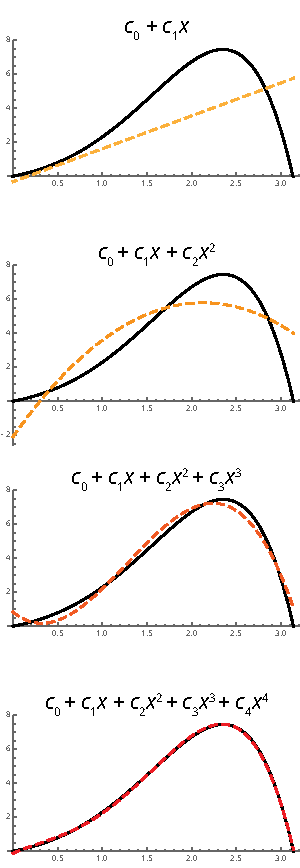
\includegraphics[width=1.75in]{img/basis_expansion.pdf}
}
\captionof{figure}{Example of expansion of the function $\exp(x) \sin(x)$ in a basis of polynomials $x^i$.
By the time we include fourth powers of $x$ this function is approximated well in the entire range $0 \leq x \leq \pi$.}
\label{fig:fit}
}
You can think of this approximation as fitting the function $g(x)$ with the basis functions, where the unknowns are the fitting coefficients $c_i$.
An important point is that, if the basis $\{ f_i(x) \}$ is chosen judiciously, the approximate solution should converge rapidly to the exact $g(x)$ when the number of basis functions ($K$) is increased.

This process is illustrated in Fig.~\ref{fig:fit}, where the function $\exp(x) \sin(x)$ is approximated with a basis of polynomials of $x$.
In this example, we stop at the polynomial of order $K$ (here we also include the constant term $x^0 = 1$)
\begin{equation}
g(x) \approx  c_0 +  c_1 x + \cdots + c_K x^{K} = \sum_{i=0}^{K} c_i x^{i}
\end{equation}
As you can see, the first two approximations are not very good, and by the time we use a forth-order polynomial we cannot easily distinguish $\exp(x) \sin(x)$ from its approximation.

\section{Gaussian-type orbitals}

To understand how we use bases in quantum chemistry we will start by learning how atomic orbitals are approximated with a Gaussian basis.
Since the early days of computational chemistry it has become common practice to approximate atomic orbitals using a basis of \emph{Gaussian functions}.
For example, if we want to approximate the 1s orbital of the hydrogen atom, $\mathrm{1s}=  \frac{1}{\sqrt{\pi}} e^{-r}$, an expansion in Gaussian functions consists of the following approximation
\begin{equation}
\frac{1}{\sqrt{\pi}} e^{-r} \approx \sum_\mu C_\mu \exp(- \alpha_\mu r^2)
\end{equation}

At this point we should ask: \emph{Why would we want to approximate a function that we already know how to write in closed form?}
The answer is that all quantum chemistry methods need to know integrals of atomic orbitals like
\begin{equation}
\int d\mathbf{r}_1 \, d\mathbf{r}_2 \, \frac{\varphi^*_i(\mathbf{r}_1) \varphi^*_j(\mathbf{r}_2) \varphi_k(\mathbf{r}_1) \varphi_l(\mathbf{r}_2)}{r_{12}}
\end{equation}
These integrals are difficult to compute with function of the form $e^{-\alpha r}$, but they turn out to be doable if one instead uses functions of the form $\exp(- \alpha r^2)$.\mnote{This is due to the Gaussian product theorem, which states that the product of two multidimensional Gaussians is still a Gaussian function.}

For each type of atomic orbital (s, p, d, etc.) one can write a corresponding \emph{Gaussian-type orbital} obtained by multiplying a 3D spherical Gaussian function $\exp(-\alpha r^2)$ times a polynomial in the coordinates $x$, $y$, and $z$
\begin{equation}
\label{eq:primitive}
x^l y^m z^n e^{-\alpha r^2}
\end{equation}
As we have seen, s orbitals are obtained from a combination of Gaussians
\begin{equation}
e^{-\alpha r^2}
\end{equation}
while p orbitals can be represented with a product of $x$, $y$, or $z$ and a Gaussian
\begin{equation}
x e^{-\alpha r^2}, y e^{-\alpha r^2}, z e^{-\alpha r^2}
\end{equation}
Atomic orbitals of d type can be formed by quadratic polynomials times a Gaussian.
In this case there are six combinations
\begin{equation}
xy e^{-\alpha r^2}, yz e^{-\alpha r^2}, xz e^{-\alpha r^2},
x^2 e^{-\alpha r^2}, y^2 e^{-\alpha r^2}, z^2 e^{-\alpha r^2}
\end{equation}
We call these 6 d orbitals \emph{Cartesian} d functions, to distinguish them from the 5 \emph{spherical} or \emph{pure angular momentum} d functions that are obtained when we solve the Schr\"{o}dinger equation
\begin{equation}
xy e^{-\alpha r^2}, yz e^{-\alpha r^2}, xz e^{-\alpha r^2},
(x^2 - y^2) e^{-\alpha r^2},  (2 z^2 - x^2 - y^2)e^{-\alpha r^2}
\end{equation}
Similarly, there are more Cartesian f functions (10) than spherical f function (7), etc.
In a quantum chemistry code, integrals are first computed using Cartesian and then these are combined to form spherical functions.
Some codes might allow you to use Cartesian or spherical functions, but you should always use the default.

\mfigure{\\
\centering{
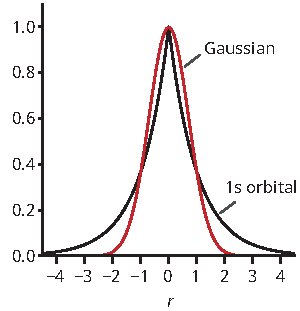
\includegraphics[width=1.75in]{img/sto_vs_gto.pdf}
}
\captionof{figure}{Plot of the STO-6G Gaussian basis set and the six Gaussian primitives for the hydrogen atom.}
\label{fig:basis:sto_vs_gto}
}

\section{Contracted Gaussian-Type Orbitals}
The Gaussians functions defined in Eq.~\eqref{eq:primitive} are also called \emph{primitives}.
Figure~\ref{fig:basis:sto_vs_gto} reports a comparison of the shape of the hydrogen 1s orbital and a 1s Gaussian primitive.
As you notice, the Gaussian and the 1s orbital are both peaked at the origin.
However, the Gaussian has a rounded top at $r = 0$ and decays too quickly when $r > 1$.
To represent the correct shape of atomic orbitals several primitives are combined together using a fixed set of coefficients to form numerically accurate approximations to atomic orbitals.
We call these function \emph{contracted Gaussians} and to avoid confusing them for orbitals, they will be denoted with the Greek letter chi ($\chi$).
For example, a p$_z$ contracted Gaussian centered at the origin is approximated as
\begin{equation}
\chi_{\mathrm{p}_z}(\mathbf{r}) = 
\sum_\mu b_\mu \, z \exp(- \alpha_\mu r^2)
\end{equation}
The quantities $\alpha_\mu$ are called the \emph{exponents} of the basis, while the coefficients $b_\mu$ are called \emph{contraction coefficients}.

A \emph{Gaussian basis set} is a collection of contracted Gaussian functions with optimized exponents and contraction coefficients.
Making a basis sets is not trivial and there are many articles in the literature describing how to build basis set.
The most commonly used basis sets are collected in the \emph{basis set exchange} on-line repository  (\url{https://www.basissetexchange.org}).

It is instructive to take a look at an example of a Gaussian basis used by a computer program.
The following shows the \emph{STO-6G} basis set for the hydrogen atom. This basis approximates one atomic orbital of hydrogen using six Gaussians (hence the ``6G'').
\mfigure{
\centering{
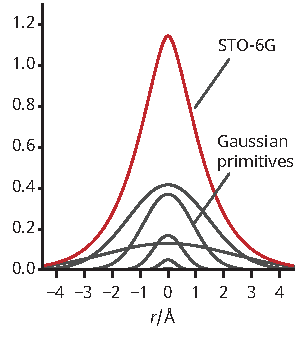
\includegraphics[width=1.75in]{img/sto-6g.pdf}
}
\captionof{figure}{Plot of the STO-6G Gaussian basis set and the six Gaussian primitives for the hydrogen atom.}
\label{fig:basis:sto-6g}
}
This basis includes only one atomic orbital for each hydrogen.
The first line lists the element name, while the second one is a tag that indicates that the next few lines show the exponent and contraction coefficients for a s-type (``S'') orbital approximated with 6 Gaussians.
The left column shows the exponent of the Gaussians, while the second column the corresponding contraction coefficients
\begin{verbatim}
H 0
S   6   1.00
      0.3552322122E+02       0.9163596281E-02
      0.6513143725E+01       0.4936149294E-01
      0.1822142904E+01       0.1685383049E+00
      0.6259552659E+00       0.3705627997E+00
      0.2430767471E+00       0.4164915298E+00
      0.1001124280E+00       0.1303340841E+00
\end{verbatim}

This basis corresponds to the function
\begin{equation}
\chi(\mathbf{r}) = 
0.009163596281 \, \exp(-35.52322122 \, r^2)
%+ 0.04936149294  \, \exp(-6.513143725 \, r^2)
+ \ldots
\end{equation}
which is plotted in Fig.~\ref{fig:basis:sto-6g}.
This figure also shows the six Gaussian primitives that are combined together to obtain the STO-6G basis function.
The STO-6G function looks like a Gaussian but it is more pointy at the origin and decays more slowly for large values of $r$.
\emph{Even though the STO-6G basis uses six Gaussians, this basis consists of only one function.}

The STO-6G basis is not a very flexible basis, since it does not allow the orbital of the hydrogen atom to shrink, grow, or polarize.
For example, if we consider the \ce{H-} anion, the STO-6G basis does not allow the occupied orbital to expand due to the increased electron-electron repulsion experienced due to the extra negative charge.
In practice, computation basis include more functions than the strict valence atomic orbitals.
For example, the def2-SVP basis for hydrogen is defined as
\begin{verbatim}
H     0
S   3   1.00
     13.0107010              0.19682158E-01
      1.9622572              0.13796524
      0.44453796             0.47831935
S   1   1.00
      0.12194962             1.0000000
P   1   1.00
      0.8000000              1.0000000
\end{verbatim}
This basis contains two s-type contracted Gaussians (SV = split valence, meaning two sets of valance orbitals) plus a set of three p orbitals (p$_x$, p$_y$, p$_z$), which are called \emph{polarization functions} (P = polarization).
Figure~\ref{fig:basis:h_def2-SVP} shows these five basis functions.
By combining orbitals $\chi_1$ and $\chi_2$ it is possible to form spherical orbitals of different size.
The p orbitals instead allow to polarize the wave function along any direction in space as shown in part \textbf{C} of this figure.

\mfigure{
\centering{
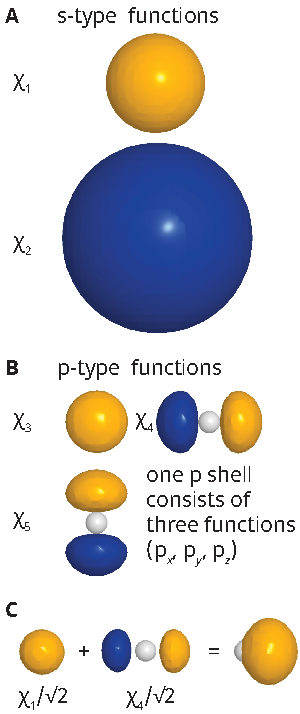
\includegraphics[width=1.75in]{img/h_def2-SVP.pdf}
}
\captionof{figure}{Plot of the def2-SVP Gaussian basis set for the hydrogen atom. (\textbf{A}) split-valence s-type functions and (\textbf{B}) p-type polarization functions.
The combination of a s-type and p-type function is a s-like function polarized along the y direction (\textbf{C}) }
\label{fig:basis:h_def2-SVP}
}

Gaussian basis sets can be built in such a way that the accuracy of the orbitals can be systematically improved.
The following table shows the energy of the hydrogen atom computed with a family of basis sets (cc--pV$X$Z, with $X = $D,T,Q,5,6) that contains an increasing number of Gaussian functions (this basis contains more than just s functions).
As you can see, the cc-pVDZ basis is already very accurate (the absolute energy error is less than 0.001 m\Eh) and the error can be reduced by almost one order of magnitude as we go from one basis to next one in this family.
\begin{center}
\captionof{table}{Convergence of the energy of the hydrogen atom as a function of the computational basis.
The exact solution corresponds to the analytic solution of the Schr\"{o}dinger equation (E = $-$0.5 \Eh).}
\begin{tabular}{@{} cccc @{}} % Column formatting, @{} suppresses leading/trailing space
\toprule
Basis    & Basis Functions & Energy (\Eh) & Error (\Eh) \\
\midrule
cc-pVDZ &   5 & $-$0.499278403 & 0.000721597 \\ 
cc-pVTZ &  14 & $-$0.499809811 & 0.000190189 \\ 
cc-pVQZ &  30 & $-$0.499945569 & 0.000054431 \\ 
cc-pV5Z &  55 & $-$0.499994535 & 0.000005465 \\ 
cc-pV6Z &  91 & $-$0.499999245 & 0.000000755 \\ 
Exact &  $\infty$ & $-$0.500000000 & 0.000000000\\
\bottomrule
\end{tabular}
\end{center}

\section{The linear combination of atomic orbitals approximation}

The Gaussian basis functions introduced in the previous section are the building blocks used to construct approximate orbitals (atomic and molecular).
A sensible choice for approximating the shape of molecular orbitals is to use a basis that is as close as possible to the atomic orbitals of isolated atoms.
The intuition here is that a lot of the details of the structure of atoms is preserved in molecules.
So it makes sense to use atomic orbitals as building blocks for approximating molecular orbitals.

This idea is called the \emph{linear combination of atomic orbitals} (LCAO).
You have already encountered LCAO when you applied molecular orbital theory to simple molecules like \ce{H2}, where the bonding orbital is the in-phase combination (superposition) of two 1s atomic orbitals, or when you were introduced to the concept of hybrid orbitals like the \ce{sp^3} hybrids of carbon in methane.
This is not the only way quantum chemistry computations are done,\mnote{Other examples include using plane waves [$\exp(i \mathbf{k} \cdot \mathbf{r})$] and numerical grids to approximate the orbitals.} but it is by far the most common approach used in most quantum chemistry programs.

Mathematically, the LCAO approximation expresses a generic orbital $\varphi_i$ as a linear combination of Gaussian basis functions $\chi_\mu$, so that
\begin{equation} \label{eq:basis:orb}
\varphi_i(\mathbf{r}) \approx \sum_\mu C_{\mu}^{(i)}\chi_\mu(\mathbf{r})
\end{equation}
The quantity $C_{\mu}^{(i)}$ is a vector of coefficients for orbital $\varphi_i$.
\emph{When you run a Hartree--Fock computation, this is the quantity that is optimized by the SCF procedure}.

For very simple molecules, the coefficients $C_{\mu}^i$ are simply determined by symmetry.
As an example, we will look at the orbitals of the \ce{H2} molecule using the STO-6G basis.
For convenience, we will label the two hydrogen atoms 1 and 2.
Each hydrogen atom carries one basis function, which we label as $\chi_1$ and $\chi_2$. These functions are shown in Fig.~\ref{fig:basis:h2_sto-6g}.	
\mfigure{
\centering{
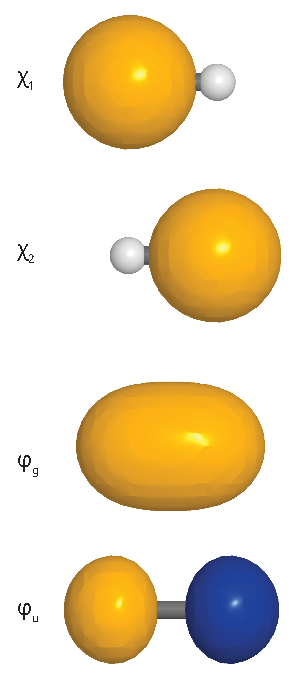
\includegraphics[width=1.75in]{img/h2_sto-6g.pdf}
}
\captionof{figure}{Hydrogen molecule. Plot of the STO-6G  basis functions ($\chi_1$ and $\chi_2$) and bonding (gerade, $\varphi_\mathrm{g}$, ) and antibonding (ungerade, $\varphi_\mathrm{u}$) molecular orbitals.}
\label{fig:basis:h2_sto-6g}
}

From these basis functions we can form two atomic orbitals.
The first one is a in-phase combination (g, from the German word \textit{gerade}) of $\chi_1$ and $\chi_2$, times a normalization factor $N_\mathrm{g}$
\begin{equation}
\varphi_\mathrm{g} = N_\mathrm{g} (\chi_\mathrm{1} + \chi_\mathrm{2}), \text{ which corresponds to }
C_1^{(1)} =  N_\mathrm{g}, C_2^{(1)} =  N_\mathrm{g}
\end{equation}
The second orbital is the out-of-phase combination (u, \textit{ungerade})
\begin{equation}
\varphi_\mathrm{u} = N_\mathrm{u} (\chi_\mathrm{1} - \chi_\mathrm{2}), \text{ which corresponds to }
C_1^{(2)} =  N_\mathrm{u}, C_2^{(2)} = -N_\mathrm{u}
\end{equation}
These are the orbitals that you will get if you do a Hartree--Fock computation on \ce{H2}.
The orbital $\varphi_\mathrm{g}$ is a \emph{bonding orbital} while $\varphi_\mathrm{u}$ is an \emph{antibonding orbital}.
Since $\varphi_\mathrm{g}$ has no nodes, its energy is lower than that of $\varphi_\mathrm{u}$.

%\emph{Note that in general if the basis set we use has $K$ functions, then a Hartree--Fock or DFT computation will generate $K$ orbitals.}\mnote{The only exception to this statement is if the basis has severe linear dependency problems.}

%
%
%and written in the form of Eq.~\eqref{eq:basis:orb} correspond to the coefficients
%\begin{equation}
%\mathbf{C}^1 = N_\mathrm{g} (1,1), \quad 
%\mathbf{C}^2 = N_\mathrm{u} (1,-1)
%\end{equation}




\section{A survey of common basis sets}

The basis set exchange website counts a total of 589 basis sets!
So how do you go about choosing the right basis set for your computation?
In choosing the right basis set we always have to balance two competing factors: the accuracy of the result and the cost of a computation.
When one is willing to tolerate a given average error, it is possible to choose a basis using previous results in the literature and use it in a study.
However, if your goal is to get the best possible result, the it might be necessary to use a range of basis sets.
By repeating computations using basis sets of increasing size, we can gauge the so-called \emph{basis set incompleteness error}, the error that arises from approximating the orbitals using a finite basis set.

For computations on large molecules with Hartree--Fock or DFT it is customary to employ a fixed basis set.
Basis sets like Pople's 6-31G, 6-311G, 6-31G*,\mnote{The 6-31G* basis set is similar to the def2-SVP basis. It is defined for the atoms H through Zn. It uses two sets of valence orbitals plus polarization functions (d-type polarization functions on atoms Li--Ca and f-type polarization functions on atoms Sc--Zn.} 6-31G**, etc. are ofter used in DFT computations on large molecules.
However, I would discourage you from using this family of basis sets because it is now obsolete and some serious problems have been discovered (e.g., when used with the MP2 method this basis gives a nonplanar structure for benzene!).

A more modern choice is the family of Karlsruhe basis sets (def2-SVP, def2-TZVP, def2-QZVP, def2-TZVPD, \ldots). For routine DFT computations, a def2-TZVP basis should provide nearly-converged results.
The ``TZV'' and ``QZV'' stand for triple zeta and quadruple zeta valence (for the Greek letter zeta, $\zeta$, often used to indicate the exponent of a Gaussian instead of the letter $\alpha$ used in these notes), that is three or four sets of valence orbitals.
``P'' and ``D'' indicate polarization and \emph{diffuse functions}, respectively.
Diffuse functions are extra Gaussian basis functions with a small exponent, which are added to a basis to give it more flexibility in the description of orbitals that are diffuse.
These functions increase the accuracy of computations on anions, long-range interactions, and excited states.

{
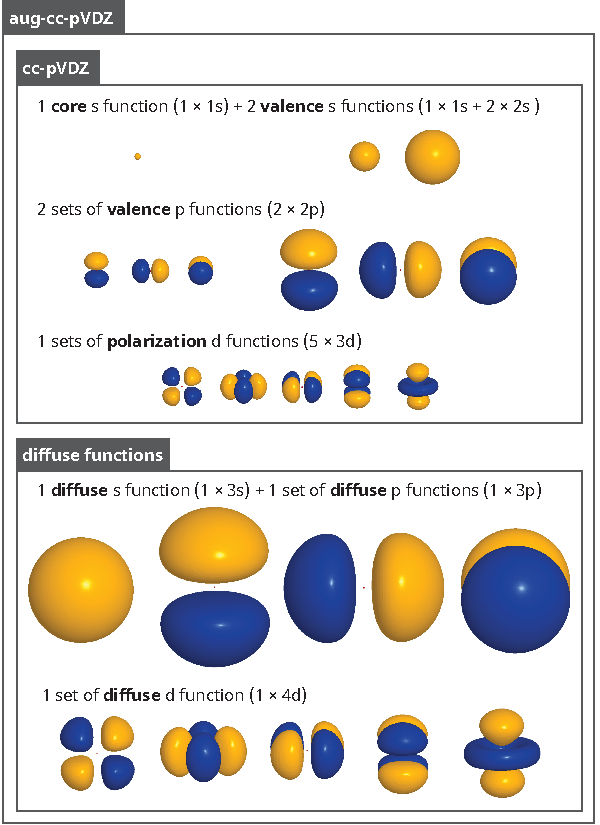
\includegraphics[width=4.00in]{img/cc-basis.pdf}
\captionof{figure}{Oxygen atom. Plot of the cc-pVDZ and aug-cc-pVDZ contracted Gaussian-type basis functions. The aug-cc-pVDZ basis is built from the cc-pVDZ by adding an extra set of diffuse functions.}
\label{fig:basis:cc-basis}
}

For wave function methods like MP2, CCSD, CCSD(T), etc., Dunning's  correlation-consistent basis sets (cc-pV$X$Z, with $X$ = D, T, Q, 5, 6) are recommended and represent the state-of-the-art.
These are families of basis sets that systematically converge to the full basis set limit.
Figure~\ref{fig:basis:cc-basis} shows the basis functions included in the cc-pVDZ basis for oxygen.
This basis includes a double set of valence orbitals (2s and 2p) and adds one set of d polarization functions.
The cc-pVDZ basis is likely to provide reasonable, but potentially inaccurate results. A cc-pVTZ basis is generally recommended for routine applications. 
For highly-accurate benchmark results it is necessary to use the cc-pVQZ or cc-pV5Z basis sets.
There are many variants of the Dunning's  correlation-consistent basis sets.
\begin{itemize}
\item The basis sets aug-cc-pV$X$Z include \emph{diffuse functions} and are useful to describe Rydberg states, long range interactions, and anions.
Figure~\ref{fig:basis:cc-basis} shows the extra diffuse functions included in the aug-cc-pVDZ basis.

\item Dunning's basis sets (cc-pV$X$Z) are meant to correlate only valence electrons, so core electrons should be frozen in computations that use them.
To account for core electron correlation it is necessary to use a \emph{core-valence basis set}, usually indicated with the symbol cc-pCV$X$Z, or the newer weighted core-valence sets (cc-pwCV$X$Z). 

\item Other variants of Dunning's basis sets include \emph{basis extended for period 3 atoms} [cc-pV($X$+d)Z], \emph{pseudopotential basis sets} for heavy elements [cc-pV$X$Z-PP], and \emph{basis sets for relativistic computations} [cc-pV$X$Z-DK].
\end{itemize}

This is by no means a comprehensive overview of basis sets.
A good practice is to use the literature as a starting point for getting a feeling for what basis sets are used by other researchers.
Ideally, before working on a project you should benchmark the convergence of the energy, the molecular geometry, or other properties that you are interested in computing using different basis sets.

Note, that \emph{it is common practice in Quantum Chemistry to cite the original reference to the basis sets employed in a computation}. Crafting a basis set for a large number of elements in the periodic table takes a lot of work and the people that invested their time doing so deserve credit for it.



\section{The complete basis set (CBS) limit and the basis set error}

To analyze the error introduced by using a finite basis we define the \emph{complete basis set (CBS) limit} as the limit of the energy (or any other property) for the basis size that goes to infinity.
\begin{equation}
E_\mathrm{CBS} = \lim_{K \rightarrow \infty} E(\text{basis of size } K)
\end{equation}
The underlying assumption is that with a \emph{complete basis} we can approximate any well-behaved function.
It is convenient to introduce the idea of the CBS limit and not just call this energy exact, because even if we use a complete basis, we are still introducing other sources of error that will make our results deviate from experiment.

The error due to the finite basis set is called the \emph{basis set incompleteness error} (BSIE).
For any method, the BSIE can be formally defined as the difference between the energy computed with a finite basis $E_\mathrm{finite\,basis}$ and the CBS limit ($E_\mathrm{CBS}$)
\begin{equation}
\Delta E_\mathrm{BSIE} = E_\mathrm{finite\,basis} - E_\mathrm{CBS}
\end{equation}

We will now take a look at the convergence of the Hartree--Fock energy as a function of the basis set for the \ce{H2+} molecule (see Table~\ref{tab:basis:h2+}). This systems has only one electron and, therefore, a Hartree--Fock computation is only affected by the error that arises from using a finite basis set.
In this case the energy converges rapidly, like in the case of the hydrogen atom.
However, the rate at which the energy converges is slower.
For example, the change in energy when going from the cc-pVDZ to the cc-pVTZ basis is only 0.53 m\Eh for H, but this number is 1.98 m\Eh for \ce{H2+}.
Comparing the energy to the best result for \ce{H2+} (cc-pV6Z basis), we conclude that cc-pVTZ is already sufficiently accurate to make quantitative predictions, and the cc-pVQZ energy is only 0.1 m\Eh (ca. 0.15 kcal/mol) off from the best result.

\begin{center}
\begin{tabular}{@{} ccc @{}} % Column formatting, @{} suppresses leading/trailing space
\toprule
Basis    & Basis Functions & Energy (\Eh) \\
\midrule
cc-pVDZ &  10 & $-$0.600264667 \\
cc-pVTZ &  28 & $-$0.602244426 \\
cc-pVQZ &  60 & $-$0.602520583 \\
cc-pV5Z & 110 & $-$0.602619758 \\
cc-pV6Z & 182 & $-$0.602632085 \\
\bottomrule
\end{tabular}
\captionof{table}{Convergence of the energy of the \ce{H2+} molecule at a bond distance $r_\mathrm{HH}$ = 2 bohr as a function of the computational basis.}
\label{tab:basis:h2+}
\end{center}




\end{document}